\documentclass[12pt]{article}

\usepackage{float}
\usepackage{enumitem}
\usepackage{graphicx}
\usepackage{hyperref}
\hypersetup{
	colorlinks=true,
	urlcolor=blue
}

\setlength{\parskip}{1ex}
\setlength{\parindent}{0pt}
\addtolength{\evensidemargin}{-0.625in}
\addtolength{\oddsidemargin}{-0.625in}
\addtolength{\textwidth}{1.25in}
\addtolength{\topmargin}{-0.625in}
\addtolength{\textheight}{1.25in}



\begin{document}
\begin{center}
\Huge\bf INFO30005 Deliverable 1
\end{center}

\subsection*{Group Details}
Group Name: \textit{Pixels}\par
Tutor: \textit{Priyankar Bhattacharjee}\par
Tutorial: \textit{Wednesday 12pm-1pm}\par
Members: \vspace{-2ex}
\begin{itemize}[noitemsep]
	\item \textit{Jeff Li 1044965}
	\item \textit{Alisa Blakeney 1178580}
	\item \textit{Noah Stammbach}
	\item \textit{Minh Hoang Phan 1068112}
\end{itemize}
\subsection*{Links}
Link to Prototype: {\small\url{https://www.figma.com/file/NWu2ItK5AM0H7M0C9MGh5Q/Assignment-1?node-id=1\%3A11}}\\
Link to Github Repository: {\small\url{https://github.com/alisay/Diabetes-Home}}
\newpage
\subsubsection*{Figma Screenshot: Patient App, no connections}
\begin{figure}[H]
	\centering
	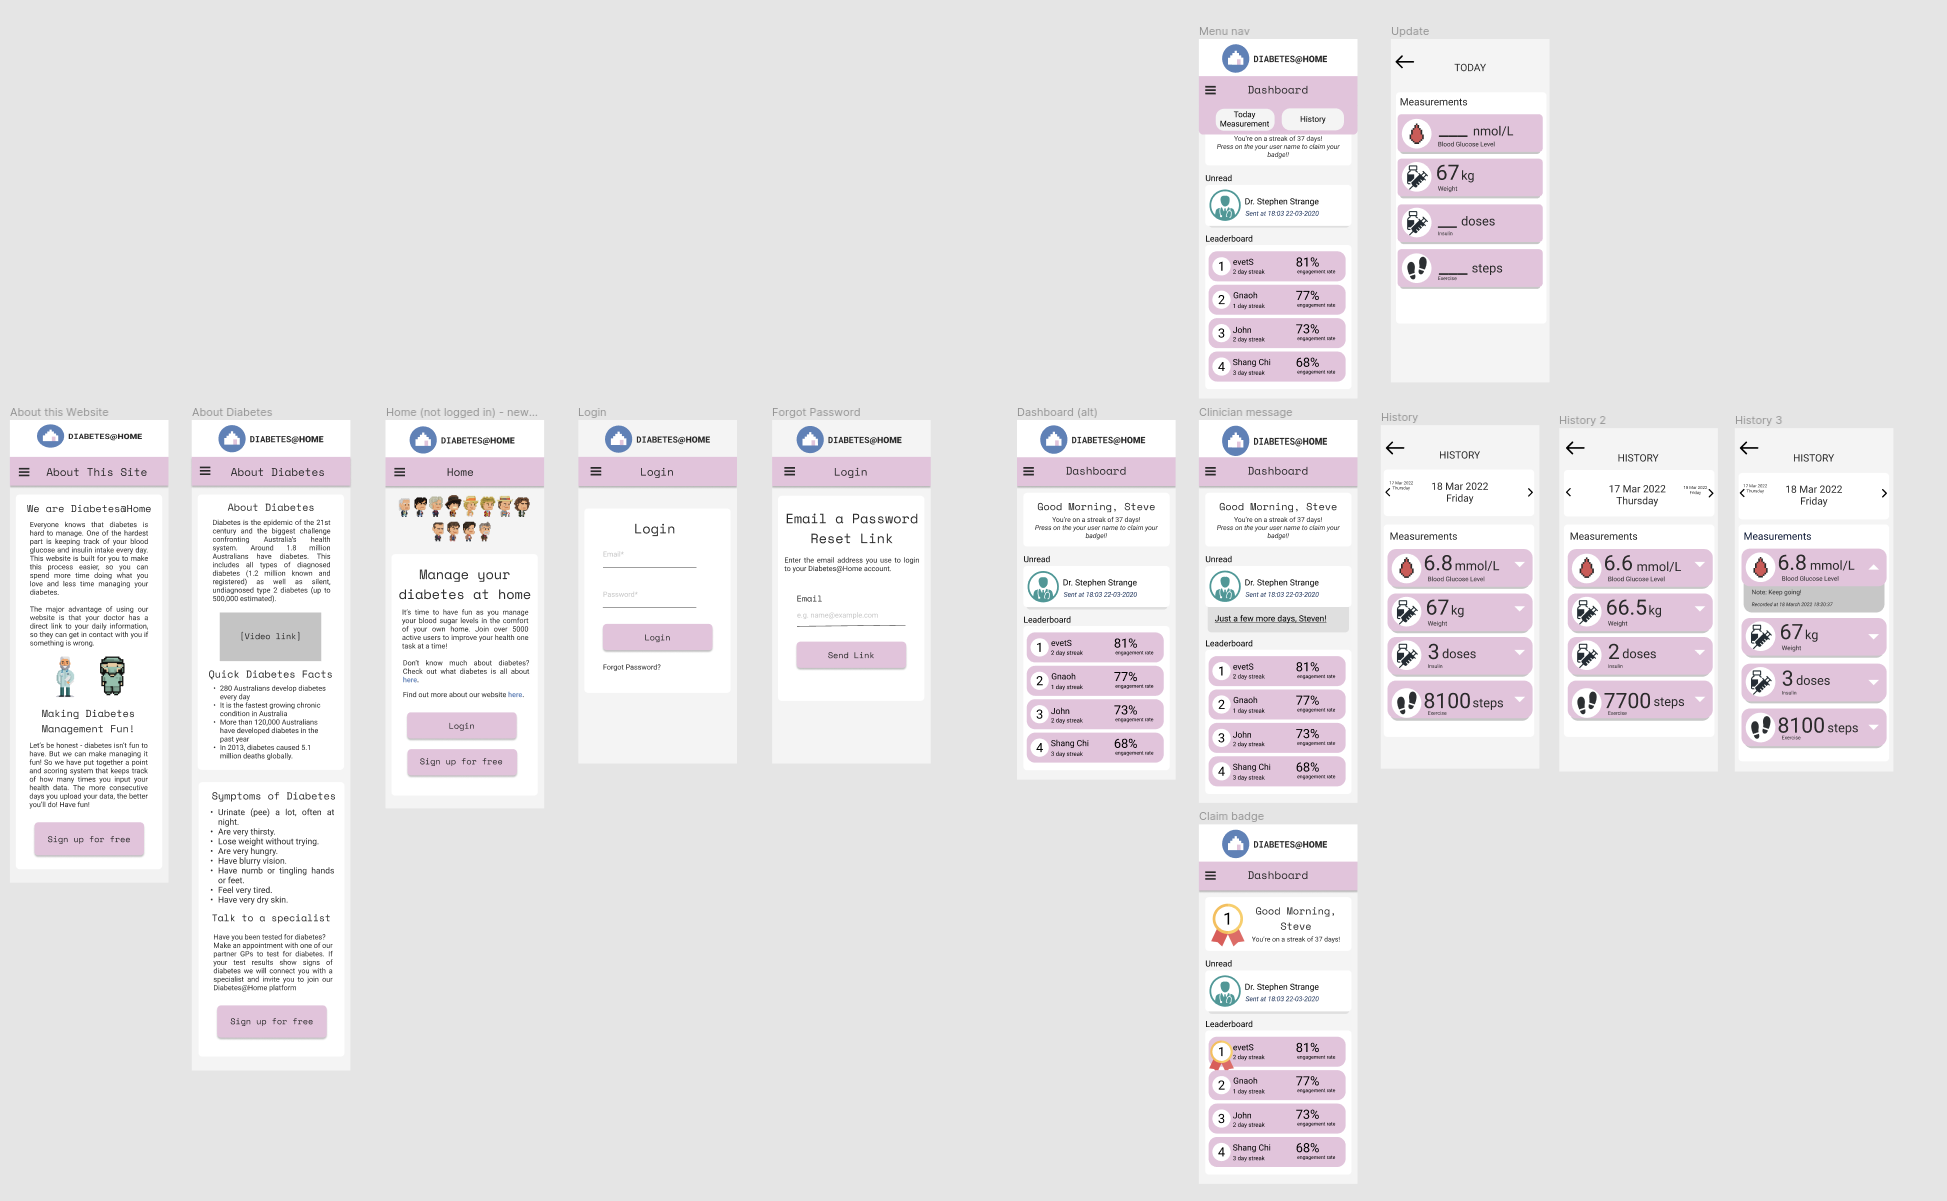
\includegraphics[width=.8\textwidth]{patient_nolines}
\end{figure}
\subsubsection*{Figma Screenshot: Patient App, with connections}
\begin{figure}[H]
	\centering
	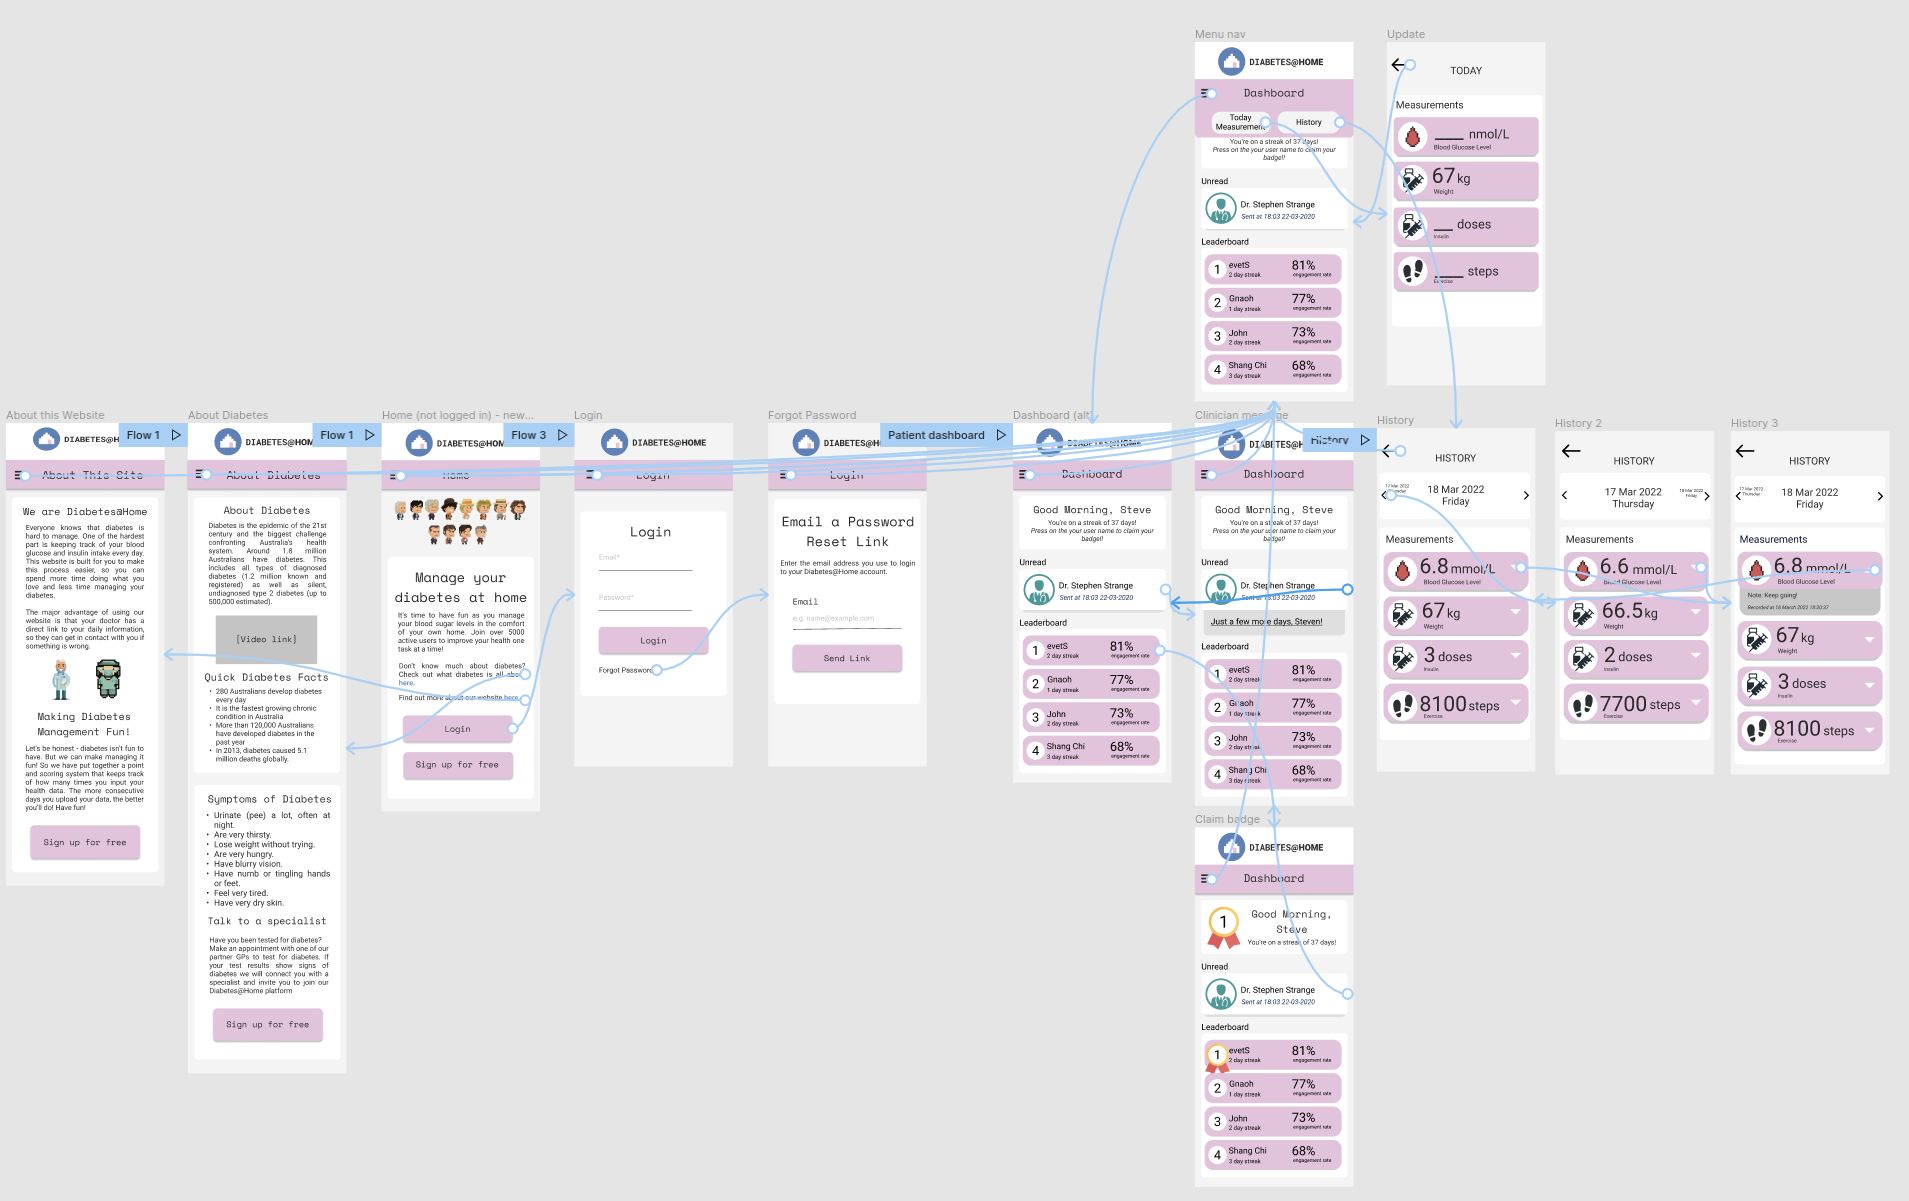
\includegraphics[width=.8\textwidth]{patient_lines}
\end{figure}\newpage
\subsubsection*{Figma Screenshot: Clinician App, no connections}
\begin{figure}[H]
	\centering
	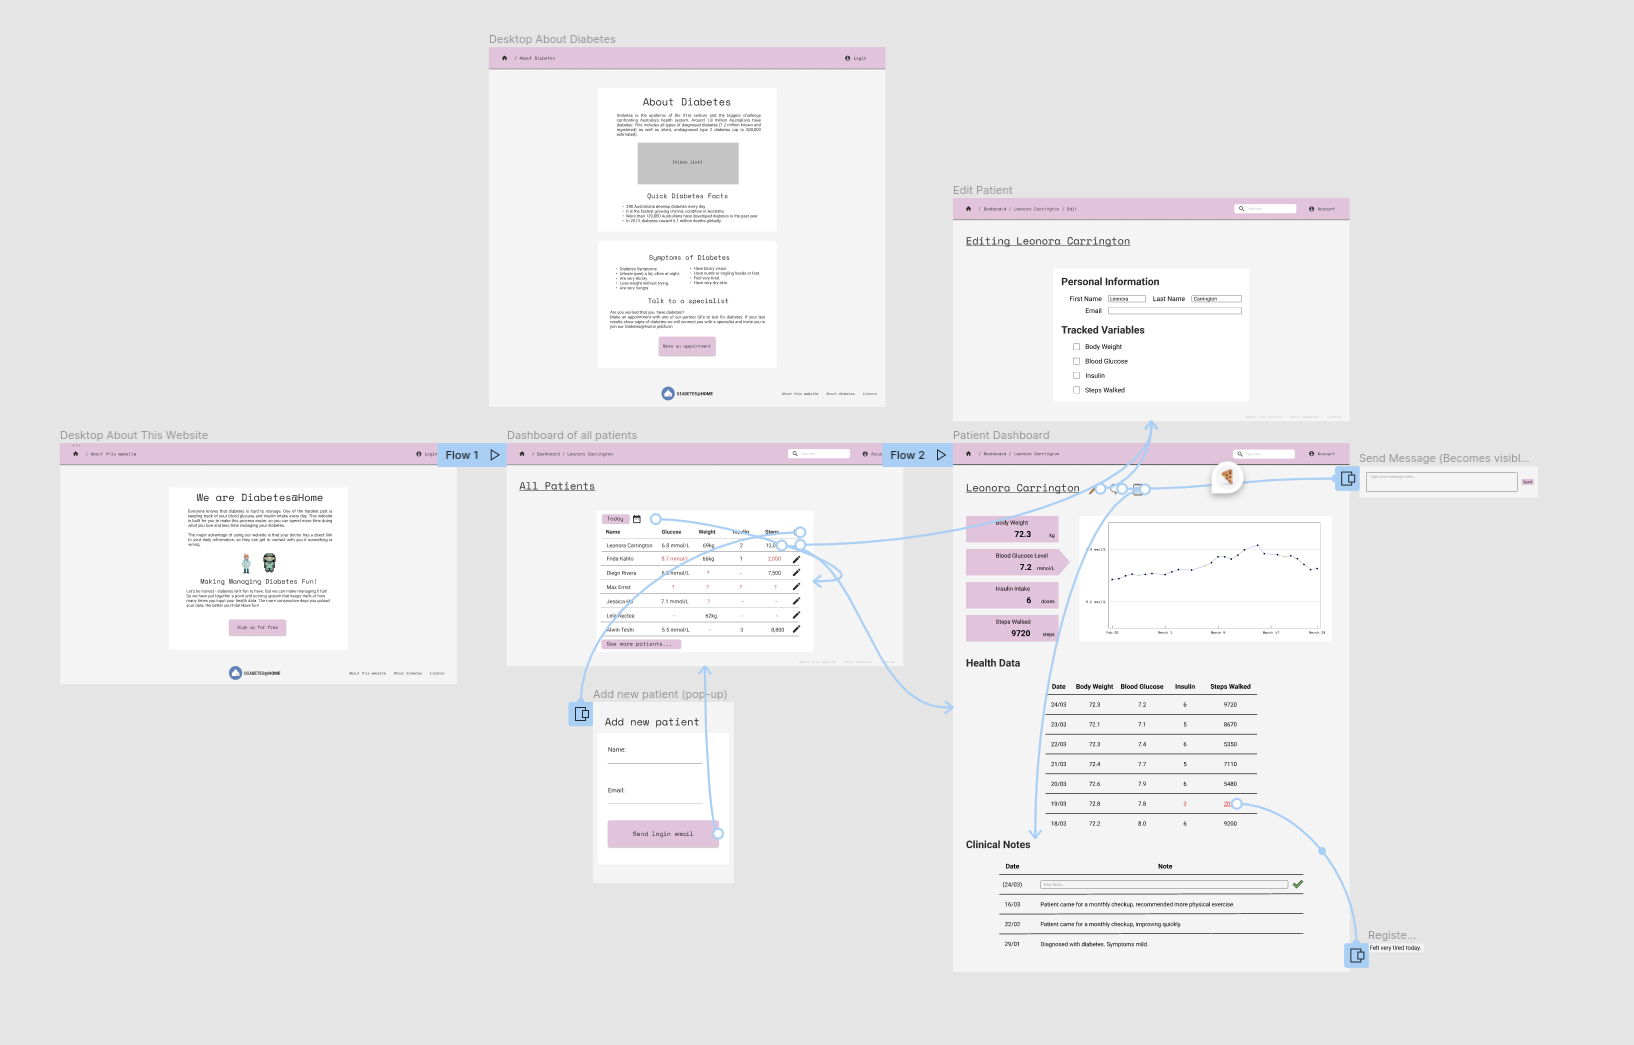
\includegraphics[width=.8\textwidth]{desktop_nolines}
\end{figure}
\subsubsection*{Figma Screenshot: Clinician App, with connections}
\begin{figure}[H]
	\centering
	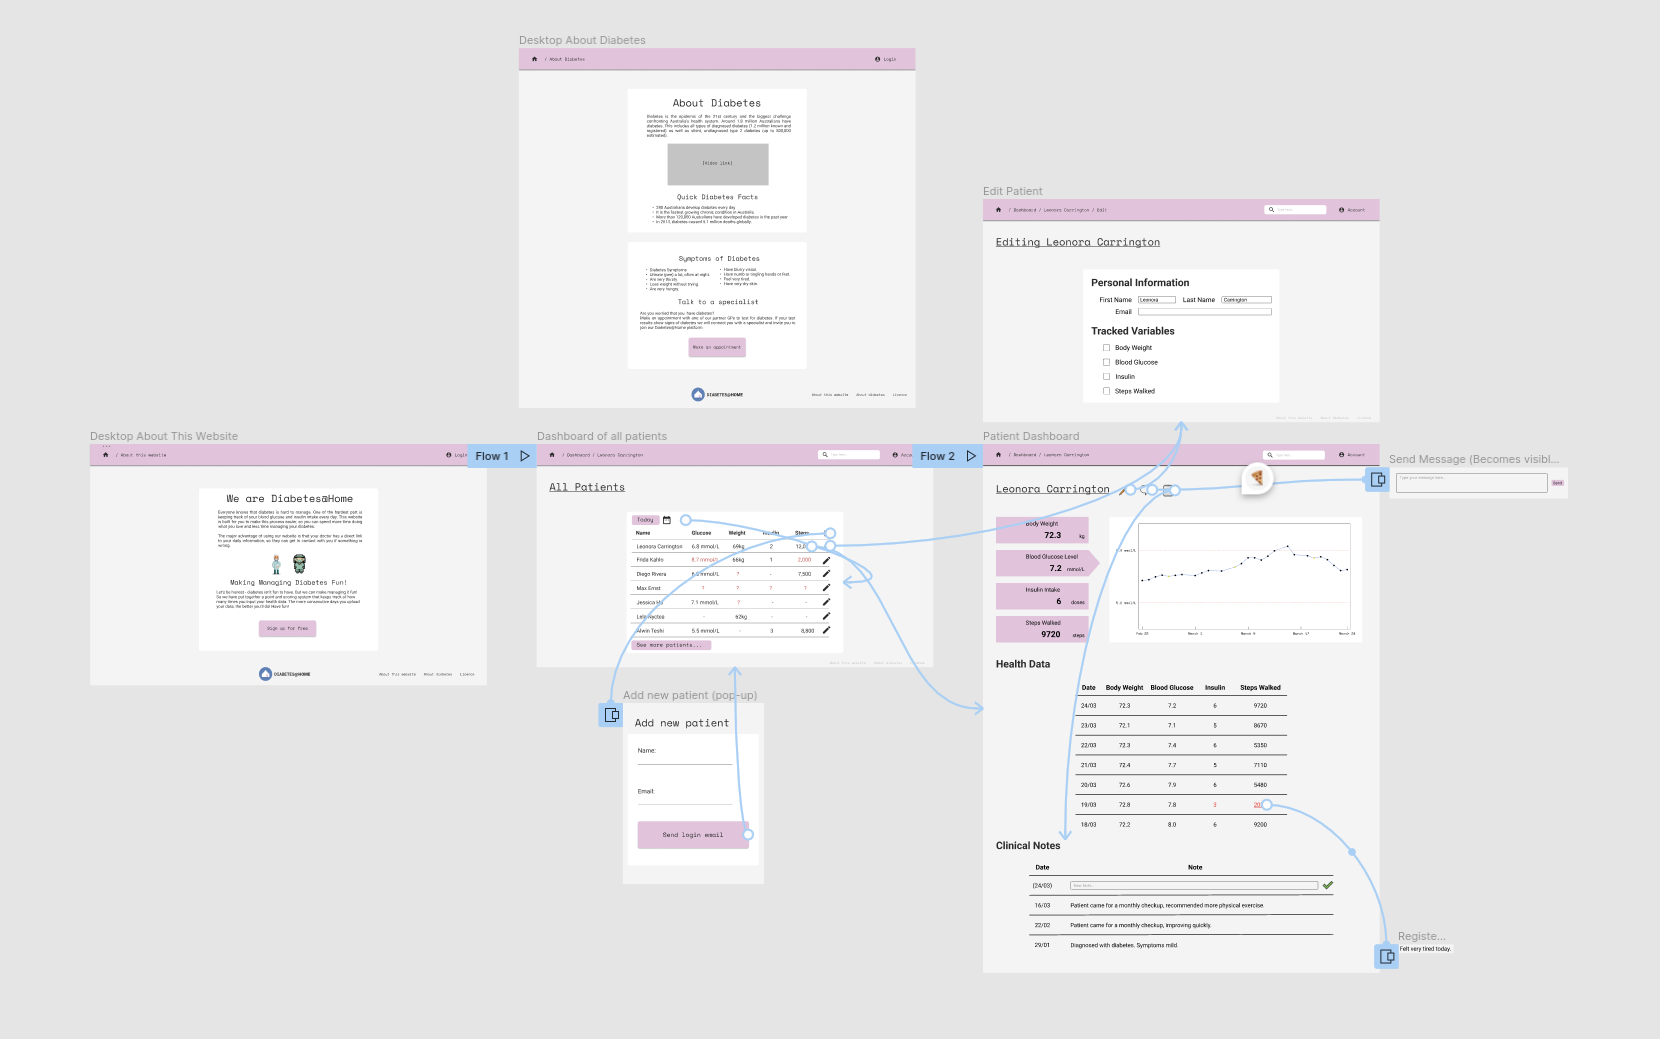
\includegraphics[width=.8\textwidth]{desktop_lines}
\end{figure}
\end{document}
